\chapter[Paper: UAV Intelligent Path Planning for Wilderness Search and Rescue]{Paper: UAV Intelligent Path Planning for Wilderness Search and Rescue\footnote {Published in IROS 2009 (IEEE/RSJ International Conference on Intelligent Robots and Systems) conference. Authors are Lanny Lin, and Michael A. Goodrich.}}
\label{chap:IROS2009}

\begin{abstract}
In the priority search phase\footnote{Four qualitatively different types of search strategies are used in WiSAR: hasty search, constraining search, priority search, and exhaustive search. See~\cite{Goodrich2008Supporting} for more details.} of Wilderness Search and Rescue, a probability distribution map is created. Areas with higher probabilities are searched first in order to find the missing person in the shortest expected time. When using a UAV to support search, the onboard video camera should cover as much of the important areas as possible within a set time. We explore several algorithms (with and without set destination) and describe some novel techniques in solving this problem and compare their performances against typical WiSAR scenarios. This problem is NP-hard, but our algorithms yield high quality solutions that approximate the optimal solution, making efficient use of the limited UAV flying time.
\end{abstract}

%=================================================================================
\section{Introduction}

The use of mini-UAVs (Unmanned Aerial Vehicles) in Wilderness Search and Rescue (WiSAR) has gained interest for researchers and experienced advancement in recent years due to its low cost, portability, and potential field use~\cite{Goodrich2008Supporting}. The UAV onboard video camera provides visual support, enables search and rescue workers to systematically survey large areas of importance in real time~\cite{Goodrich2008Supporting,Quigley2005Towards}, and increases the workers' awareness of the environment.

For WiSAR, as time progresses, the survivability of the missing person decreases and the effective search radius increases by approximately 3km/hour~\cite{Setnicka1980Wilderness,Syrotuck2000Introduction}. Therefore, search efficiency can dramatically affect the outcome of the search and rescue. In the prioritized search phase, the incident commander creates a probability distribution map for finding the missing person based upon terrain features, profile of the missing person, weather conditions, and subjective judgment of expert searchers. Such maps can also be created systematically by utilizing geographical information available to the public via the Internet~\cite{Lin2009Bayesian,Ferguson2008GIS,Soylemez2006Utility}. UAVs have limited flying time, and in most cases, it is not long enough for the onboard video camera to cover the entire search area. For these reasons, the important question is this: given a probability distribution map, a starting point, an ending point (optional), and specified flying time, what is the best path that enables the UAV onboard video camera to ``cover'' as much of the probability distribution as possible?

Characteristics such as possibly repeated visits and probability cumulation make this a more challenging problem than standard Orienteering Problem (OP) and coverage problem. Contributions of this paper include novel path planning techniques (``global warming effect'', path crossover/mutation), additional specified-destination constraint while accumulating probability, a solid validation of the algorithms' performance, and applying algorithms to a practical, real-world application. Experimental results from this paper are conducted in simulation and not on-board a real UAV. 

%=================================================================================
\section{Problem Formulation}

We model this problem as a discretized combinatorial optimization problem with respect to probability accumulated in the 2D space for UAVs that use gimbaled cameras. Using Koopman's search metric of the instantaneous probability of detection by one glimpse~\cite{Koopman1980Search}, we assume the observer has a 100\% target detection rate. This means that as the UAV camera footprint moves along the probability distribution map, it collects (``zeros out'') all the probability along the way and accumulates the probability. A good analogy would be thinking of the UAV as a vacuum cleaner sucking up probabilities with 100\% efficiency.

In WiSAR operations, a UAV maintains an altitude of approximately 60m above ground and travels at roughly 12--13m/s~\cite{Goodrich2008Supporting}. With this height, the onboard camera footprint size comes to about 32m$\times$24m. The batteries on the UAV can keep it airborne for approximately 1--2 hours depending on weather conditions. We assume that the UAV will always maintain the same height of 60m above ground (through Height-Above-Ground automation) and travel at the constant speed of 12m/s, and use 24m$\times$24m as the effective camera footprint size. Given these parameters, a 60$\times$60 probability grid, where each probability node is 24m$\times$24m, represents an area of 2.0736km$^2$ that will take the UAV 2~hours to cover entirely. In our path planning, we restrict the direction a UAV can travel to only North, South, West and East (making only 90 degree turns), and it takes the UAV 2~seconds (1~time step) to travel from one node to its direct 4-connected neighbor. In real flights, a UAV can approximate a 90~degree turn (covering 3~nodes) in 4~seconds, so this model is close to UAV's capabilities. Also during roll or yaw, the gimbaled camera can rotate to remain aiming straight down, enabling the 90 degree turn of the camera footprint.

Using $i$ for the row number and $j$ for the column number, each probability node (cell in grid) can be written as $N_{ij}$ where $0{\leq}i,j{<}60$. The value of each $N_{ij}$ is the total volume of probability within the grid cell and thus
\begin{equation}
\sum_{i=0}^{n-1}\sum_{j=0}^{n-1}N_{ij} = 1,
\label{4totalP}
\end{equation}
where $n$=60. Let $T$ be the total number of time steps allowed for the UAV (specified flying time). Let $P$ be the set of all possible paths for the UAV on the probability grid for $T$ time steps. Each path, $p_{k} \!{\in} P$, can be represented by a sequence of probability nodes \{$N_{0},N_{1},N_{2},...,N_{T}$\} consisting of $T\!{+}1$ nodes. If the UAV is allowed to visit a node more than once, then the same node can be in a different part of the sequence.

If we use a binary variable $x_{ij}$ to represent whether $N_{ij} \!{\in} p_{k}$, $x_{ij}$ becomes a function of path $p_{k}$: 
\begin{equation}
x_{ij}(p_{k}) = 
	\left\{
	\begin{array}{cl}
		1, & N_{ij} \in p_{k} \\
		0, & \mbox{otherwise}
	\end{array}
	\right.
\label{inpath function}
\end{equation}
The number of unique nodes visited is less than or equal to the length of the path:
\begin{equation}
\sum_{i=0}^{n-1}\sum_{j=0}^{n-1}x_{i,j}(p_{k}) \leq T + 1,
\end{equation}
and the total probability accumulated, $PC_{p_{k}}$, if the UAV follows path $p_{k}$ is
\begin{equation}
PC_{p_{k}}=\sum_{i=0}^{n-1}\sum_{j=0}^{n-1}x_{ij}(p_{k})N_{ij}.
\label{pathk}
\end{equation}

The optimal path $p^* \!{\in} P$ is defined such that $\!{\forall} p_{k} \!{\in} P, PC_{p^*} \!{\geq} PC_{p_{k}}$, and our goal is to find or approximate the path $p^*$, which produces the maximum cumulative probabilities within reasonable computation time.

%=================================================================================	
\section{Related Work}

Many algorithms have been used for UAV path planning such as Voronoi Diagram with Eppstein's $k$-best paths algorithm ~\cite{Beard2005Autonomous}, A*~\cite{Quigley2005Towards}, LRTA*~\cite{Howlett2006Learning}, and Probability Roadmaps~\cite{Pettersson2006Probabilistic}. These papers focus on obstacle avoidance and sensing multiple targets. 

For path planning in searching for a target, some researchers propose to use a probabilistic model and try to maximize accumulated probability along the path. In~\cite{Hansen2007Probabilistic}, Hansen et al.\ propose three search strategies: greedy, contour, and composite search, using a probability grid. In a series of papers (e.g.~\cite{Bourgault2006Optimal,Bourgault2008AugmentedNodes}), Bourgault et al.\ describe a Bayesian framework for trajectory planning to maximize the chances of finding the target given restricted time using one or multiple UAVs and human systems. However, the solution uses a very simple 1-step lookahead approach which generates paths far from optimal and difficult to improve upon. Both papers do not consider the possible set destination constraint and also lack solid validation of the path efficiency.

If we disallow visiting the same node more than once, this problem falls within a variation of the Traveling Salesman Problem (TSP) called the Orienteering Problem (OP)~\cite{Ramesh1992Optimal} or the Prize-Collecting Traveling Salesman Problem (PCTSP)~\cite{Gutin2002Traveling}, both of which are NP-Hard~\cite{Sokkappa1990Cost}. Many exact solving methods for the OP have been developed~(\cite{Laporte1990Selective,Fischetti1998Solving,Ramesh1992Optimal}. These exact methods can find optimal solutions to small OP problems, but for large-scale OP problems, approximation heuristic approaches are preferred. Mittenthal and Noon~\cite{Mittenthal1992Insert} present a heuristic approach that inserts or deletes a city from the subset-tour. Tasgetiren and Smith propose a Genetic Algorithm in~\cite{Tasgetiren2000Genetic} that encodes tours using a sequence of points and uses a penalty function to help search infeasible regions. Liang and Smith present an Ant Colony Optimization approach that uses an unusual sequenced local search and a distance-based penalty function in~\cite{Liang2006Ant}. These algorithms work well with OP problems of small number of nodes (21--100 nodes) but can be slow with large number of nodes. They also don't allow repeated visits.

%=================================================================================	
\section{Path Planning Algorithms}

Because none of the path-planning algorithms we discussed above work well under our model of the problem, we developed a set of algorithms based on the following ideas: Local Hill Climbing (LHC), Convolution, and Evolutionary Algorithms (EA). We also verify the paths generated to ensure the UAV is not flying backward or going outside of the allowed search area.

\subsection{Algorithms without a Set Destination}

In situations where the operator does not have a preference for where the path should end, the following algorithms were built and evaluated.

%=============================
\subsubsection{Complete-coverage Algorithm (CC)}

The algorithm plans flight paths by following a lawnmower pattern. It first identifies the smallest $m \!{\times} n$ bounding rectangle that contains all the non-zero probability nodes. If the starting location is inside the pattern, the algorithm simply generates a path following the pattern. Otherwise, it first plans a shortest path to the edge of the bounding rectangle. When allowed flight time is large enough, this algorithm is guaranteed to collect all the probabilities.

%%=============================
%\subsubsection{Potential Fields Algorithm}
%
%The Potential Fields (PF) algorithm is based on techniques from behavior-based robotics~\cite{[06PotentialFields]Arkin}. In our implementation, each probability node emits an attractive field with a discounting factor $\gamma$, which is a function of the distance between the node and the UAV's current position. Because we are using a 4-connected approach, Manhattan distance is used, and each node emits equal attractive forces both North-South and East-West. The discounted force $f$ can be calculated as: $f = \gamma N_{ij}$, where the discounting factor $\gamma = e^{\frac{-d^{2}}{2\sigma^{2}}}$, $d$ is the distance and $\sigma$ is the standard deviation of a scaled Gaussian curve. Attractive forces in all four directions of the UAV's current position are evaluated, and the UAV follows the direction of the strongest force. In case of a tie, a random direction is selected from the tied directions. The algorithm runs the PF algorithm multiple times with $\sigma \!{=} 10, 20, ..., 120$ and then returns the best path found.

%The discount function plot is shown in Figure~\ref{PFCurves}.
%
%\begin{figure}
%\centering
%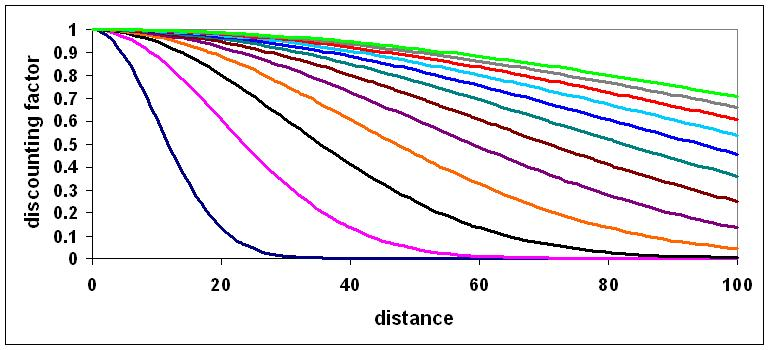
\includegraphics[width=3.5in]{PFCurves.jpg}
%\caption{Potential Field forces discount function with $\sigma=10,20,...,120$}
%\label{PFCurves}
%\end{figure}

%=============================
\subsubsection{Local Hill Climbing Algorithms (LHC)}

This is a greedy algorithm that always follows the direction with the highest value. A direct implementation of LHC does not work well with a multi-modal probability distribution map because the path generated stays with one mode until it has covered it completely before moving on to another. To address this problem, we use a global warming metaphor where the ``ocean surface'' represents all the zero-valued nodes and the ``islands'' represent the probability modes; see Fig.~\ref{GlobalWarming}. We subtract a constant $C$ from all nodes but keep all node values non-negative, where $C \!{=} \max{(N_{ij})}/l$, and $l$ defines how fine grained the search should be:
\begin{equation}
N_{ij}' \leftarrow
	\left\{
	\begin{array}{ll}
		N_{ij} - C, & N_{ij} > C \\
		0, & \mbox{otherwise}
	\end{array}
	\right.
\label{4GW}
\end{equation}
When the ocean surface rises $C$ each time, the volume of islands above water decreases, and if the ocean surface rises $l$ times, all islands will be below water. In our experiments we set $l$=40 and use the LHC algorithm to generate 40 paths: one before the ocean surface rises and one for each time the ocean surface rises (before water covers everything). We then recompute the probability accumulated for these 40 paths using the original probability grid and return the best path. This global warming technique allows the LHC algorithm to break out of one mode before completely covering that mode and move toward another. In case of a tie as to where to go next, we use two methods as the tie-breaker: LHC-GW-CONV uses a convolution kernel (with small, medium and large sizes) to determine which neighbor is more promising, and LHC-GW-PF uses Potential Fields (PF) with various discounting factors to determine where to go next.

\begin{figure}
\centering
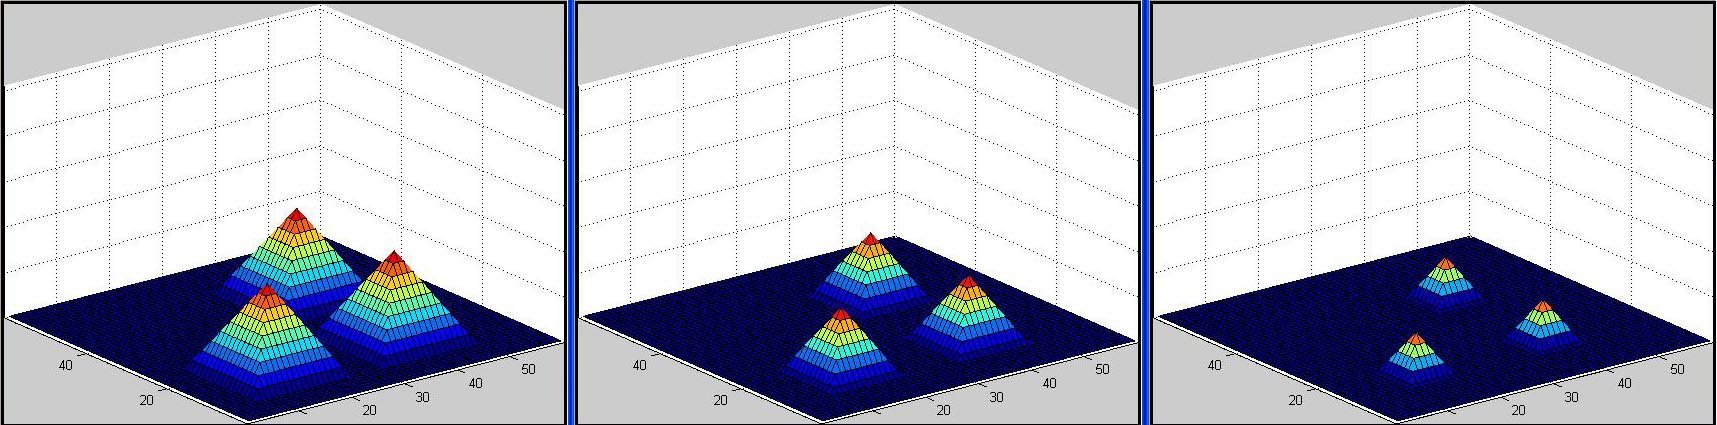
\includegraphics[width=6in]{GlobalWarming.jpg}
\caption{Global Warming Effect}
\label{GlobalWarming}
%\vspace*{-3ex}
\end{figure}

%=============================
\subsubsection{Evolutionary Algorithms}

We developed two Evolutionary Algorithms: EA-Dir and EA-Path. Both use the probability accumulated for each path as the fitness function and employ the proportional selection method~\cite{Mitchell1997Machine}. The difference between the two algorithms lies in the path representation during crossover.

With the EA-Dir algorithm, a path is encoded as a string of directions consisting of North, East, South, and West in the crossover phase (e.g. ``NNWEE...''). Because the paths generated using single-point crossover~\cite{Mitchell1997Machine} have a very high probability of being invalid (flying out of the map), we only use double-point crossover~\cite{Mitchell1997Machine} and restrict the mid-section to a fixed 5-direction string.

With the EA-Path algorithm, a path is encoded as a sequence of node positions. If the two parent paths share only one common node, then single-point crossover is used; if they share two common nodes in the same order, then double-point crossover is used; otherwise, the two parent paths are discarded and the process starts over. For the single-point crossover method the two parent paths are crossed at the common node; see Fig.~\ref{CType1}. For double-point crossover method, the first common node and the second common node in the parent paths mark the middle sections to be swapped; see Fig.~\ref{CType2}. Both techniques could result in one longer path and one shorter path. The longer path is truncated back to the original path length and the shorter path is extended by performing crossover again and then truncating.

\begin{figure}
\begin{tabular}{cc}
\begin{minipage}[b]{0.4\linewidth}
\centering
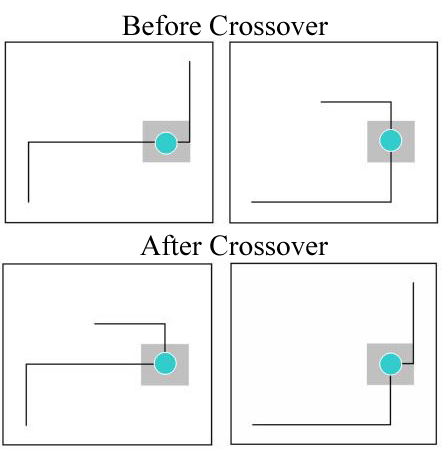
\includegraphics[width=2.5in]{crossover1.jpg}
\caption{An example of single-point path crossover (Upper row: the parents. Lower row: the children)}
\label{CType1}
\end{minipage}
\hspace{1cm}
\begin{minipage}[b]{0.4\linewidth}
\centering
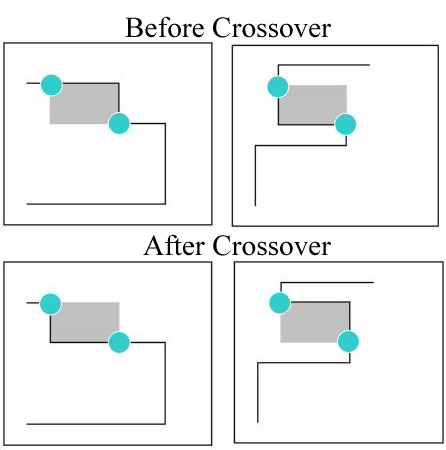
\includegraphics[width=2.5in]{crossover2.jpg}
\caption{An example of double-point path crossover (Upper row: the parents. Lower row: the children)}
\label{CType2}
\end{minipage}
\end{tabular}
%\vspace*{-4ex}
\end{figure}

Two types of mutation methods~\cite{Mitchell1997Machine} are used for flight path evolution; see Fig.~\ref{Mutation}. They follow a greedy approach with the hope that small positive changes to the path will lead to larger positive changes to the path. First we randomly select a node in the flight path and see if the next two nodes along the path would form an L shape with this node or a straight line (these are the only two possibilities). In the first case, method~1 (``flip'') is used and the algorithm replaces the middle node with the node that mirrors the middle node if we connect the first node and the third node with a line. This is like flipping a section of the path. In the second case, method~2 (``pull'') is used and the algorithm inserts two nodes into the path on one side of the line next to the first and the second nodes. This effectively extends the path by two nodes, so we simply truncate the last two nodes from the path. This is like pulling a string from the middle when the beginning end of the string is fixed. Which side to select for insertion depends on whether the new path is a valid path. If both sides allow valid paths, then the algorithm prefers inserting nodes that are not already in the path. Random selection is the last tie-breaker. If all four nodes on either side of the line are already included in the path, then a new mutation point is randomly selected and the same procedure repeats.

%\begin{figure}
%\begin{tabular}{cc}
%	\begin{minipage}{0.25\textwidth}
%	\flushright 
%	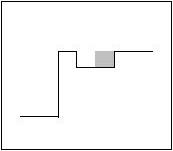
\includegraphics[width=1in]{m1_1.jpg}
%	\end{minipage}
%	\begin{minipage}{0.25\textwidth}
%	\flushleft
%	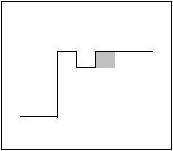
\includegraphics[width=1in]{m1_2.jpg}
%	\end{minipage}\\
%\end{tabular}
%\begin{tabular}{cc}
%	\begin{minipage}{0.25\textwidth}
%	\flushright 	
%	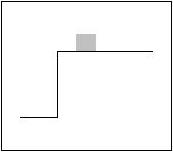
\includegraphics[width=1in]{m2_1.jpg}
%	\end{minipage}
%	\begin{minipage}{0.25\textwidth}
%	\flushleft
%	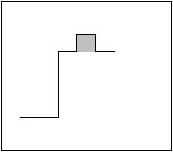
\includegraphics[width=1in]{m2_2.jpg}
%	\end{minipage}\\
%\end{tabular}
%\caption{Before and after mutation. (Upper: method 1. Lower: method 2)}
%\label{Mutation}
%\end{figure}

\begin{figure}
\begin{tabular}{cc}
\begin{minipage}[b]{0.40\linewidth}
\centering
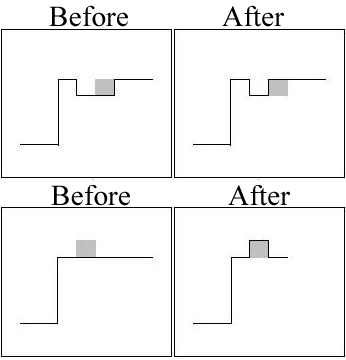
\includegraphics[width=2.5in]{mutation.jpg}
\caption{Examples of mutations in EA-DIR and EA-Path algorithms. (Upper row: method 1. Lower row: method 2)}
\label{Mutation}
\end{minipage}
\hspace{1cm}
\begin{minipage}[b]{0.40\linewidth}
\centering
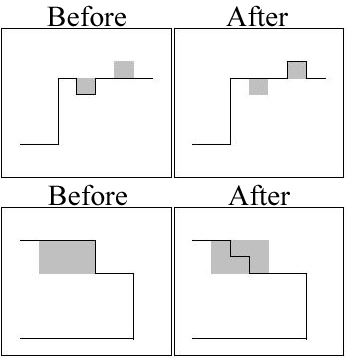
\includegraphics[width=2.5in]{mutationE.jpg}
\caption{Examples of mutations in EA-Path\_E algorithm. ~\\ (Upper row: method 2. Lower row: method 3)}
\label{MutationE}
\end{minipage}
\end{tabular}
%\vspace*{-4ex}
\end{figure}

We use an initial population of 100 paths including various paths generated using other algorithms and 95 randomly generated paths. LHC-GW-PF is not used because it is too slow. Other parameters include replacement rate at 30\% and mutation rate at 50\%. The best three paths are always kept in each iteration. The algorithm runs for at least 500 iterations and stops if either the best path does not improve after 200 iterations or if the algorithm has completed 1000 iterations.


%=================================================================================	
\subsection{Algorithms with a Set Destination}

In WiSAR, an operator might prefer the path to end at a specific destination node to support UAV retrieval, persistent visualization of a specific region at a specific time, or planning multiple path segments that make up a longer path. The following algorithms are modified versions from the previous section to handle the additional requirement. We simply add ``\_E'' to the algorithm names to distinguish them.

%=============================
\subsubsection{Complete-coverage Algorithm (CC\_E)}

This algorithm is identical to the CC algorithm up to the time when the remaining flight time is just enough to fly the UAV to the end node, then it flies toward the end node using the LHC-GW-CONV\_E algorithm (discussed shortly).

%%=============================
%\subsubsection{Potential Fields Algorithm}
%
%The PF\_E algorithm is similar to the PF algorithm except it is more constrained. During path generation, when choosing which node to go next, if going to the node makes it impossible to get to the end node within the remaining flight time, the node will not be selected. This simple constraint causes the algorithm to generate a path that allows the UAV to arrive at the end node at exactly the end of the specified flight time.

%=============================
\subsubsection{Local Hill Climbing Algorithms}

The LHC-GW-CONV\_E and LHC-GW-PF\_E algorithms have an additional constraint where nodes that prevent the path from reaching the end node within the remaining time will not be selected.

%=============================
\subsubsection{Evolutionary Algorithm}

The direction representation of a path does not work with a set destination, so the EA-Path\_E algorithm also uses a sequence of node positions to encode the path. Here we increased mutation rate to 90\% to force more exploration of the state space. The initial population of 100 paths includes various paths generated using other algorithms as seeds (both from start node to end node and reversed) and 90 randomly generated paths.

The EA-Path\_E algorithm uses both single-point and double-point crossover. The difference is that when the child path is too long, the algorithm truncates the path to the original path length, then backtracks the path until the distance between the end of the child path and the desired end node matches the remaining time. The LHC-GW-CONV\_E algorithm is then used to complete the path with the desired end node. If the child path is too short, the LHC-GW-CONV\_E algorithm is used to complete the path.

The EA-Path\_E algorithm uses three types of mutation methods. First, we randomly select a node in the path and see if the next two nodes along the path would form an L shape with this node or a straight line. In the first case, method~1 (``flip'') is used (identical to the one used in the EA-Path algorithm); see Fig.~\ref{Mutation}. If the nodes form a straight line, then method~2 (``pull'') or 3 (``shake'') is selected with equal probabilities; see Fig.~\ref{MutationE}.

Mutation method~2 (``pull'') is a modified version from the EA-Path algorithm. This method does not truncate two nodes at the end of the path; instead, it deletes two nodes in the middle of the path. This is like pulling a string from the middle when both ends of the string are fixed.

Mutation method~3 (``shake'') works by first marking a small mid-section in the path (to keep it short, we set it to 6 nodes). We first randomly select a node in the path, then traverse the path and find the fifth node down the path. If the path between these two nodes is not a straight line, the method replaces the mid-section with random flying while maintaining the same length for the mid-section. This is similar to shaking a chain where the beginning and ending points remain fixed but the middle section shifts.

%\begin{figure}
%\begin{tabular}{cc}
%	\begin{minipage}{0.25\textwidth}
%	\flushright 
%	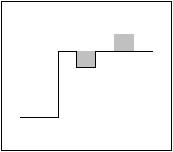
\includegraphics[width=1in]{mE2_1.jpg}
%	\end{minipage}
%	\begin{minipage}{0.25\textwidth}
%	\flushleft
%	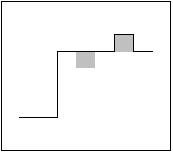
\includegraphics[width=1in]{mE2_2.jpg}
%	\end{minipage}\\
%\end{tabular}
%\begin{tabular}{cc}
%	\begin{minipage}{0.25\textwidth}
%	\flushright 	
%	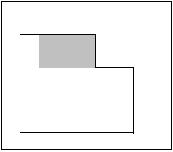
\includegraphics[width=1in]{mE3_1.jpg}
%	\end{minipage}
%	\begin{minipage}{0.25\textwidth}
%	\flushleft
%	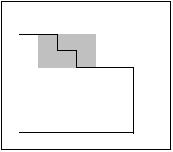
\includegraphics[width=1in]{mE3_2.jpg}
%	\end{minipage}\\
%\end{tabular}
%\caption{Before and after mutation. (Upper: method 2. Lower: method 3)}
%\label{MutationE}
%\end{figure}


%=============================
\section{Experimental Results and Analysis}

%=============================
\subsection{Performance Metrics}

We use $\mathit{Efficiency}$, $\mathit{Efficiency_{LB}}$ and Running Time as metrics to measure the performance of the algorithms, where $\mathit{Efficiency}$ is calculated if we know what's the best possible and $\mathit{Efficiency_{LB}}$ is used as an estimation when we have no way of calculating the best possible. Sorting all the probability nodes by their values in descending order would generate a list \{$N_1, N_2, N_3, ..., N_{3600}$\}. For the best possible path $p^*$, the probability accumulated $PC_{p^*}$ is constrained by a theoretical upper bound $B$:
\begin{equation}
PC_{p^*} \leq \sum_{n=1}^{T+1-d}N_n = B,
\label{topN}
\end{equation}
where $d$ is the distance from the start node to the closest non-zero valued node. Then for any path $p_k$, we define $\mathit{Efficiency}$ and $\mathit{Efficiency_{LB}}$ as the following:
\begin{equation}
\mathit{Efficiency} = \frac{PC_{p_k}}{PC_{p^*}}
\label{4Efficiency}
\end{equation}
\begin{equation}
\mathit{Efficiency_{LB}} = \frac{PC_{p_k}}{B}
\label{4EfficiencyLB}
\end{equation}
$PC_{p_k}$ can be calculated using~(\ref{pathk}). $\mathit{Efficiency}$ can be calculated when $PC_{p^*}$ is known and $\mathit{Efficiency_{LB}}$ can be calculated anytime. Clearly, $\mathit{Efficiency_{LB}} \leq \mathit{Efficiency}$.

For example, a path with 95\% $\mathit{Efficiency}$ means the amount of probability accumulated following this path is 95\% of the maximum possible. A path with 85\% $\mathit{Efficiency_{LB}}$ means the probability accumulated is 85\% of the maximum amount possible if the UAV can teleport from node to node, and the true $\mathit{Efficiency}$ could be much higher.

All experiments are run on a Dual-core AMD 3800+ PC with 1GB of memory. For each algorithm, running time is recorded so we can compare algorithm speed.


%=============================
\subsection{Typical WiSAR Scenarios}

In our experiments, we focus on probability distribution maps of three abstract but representative WiSAR scenarios: unimodal, bimodal, and bimodal with overlap. The top row of Fig.~\ref{maps} shows the 2D representations where each pixel is a probability node; the lighter the pixel, the higher the probability value. The middle row shows three simplified versions of the distributions, which can be used to manually identify the best path possible for each map and compute $PC_{p^*}$. Then we can measure the true $\mathit{Efficiency}$ of paths generated. The blue arrows on the maps mark the starting node (possible location for a WiSAR command center) and the red dots mark the ending node (intentionally selected at a different region from the starting nodes). The bottom row shows the best paths generated for the real maps at $T$=900.

\begin{figure}
\centering
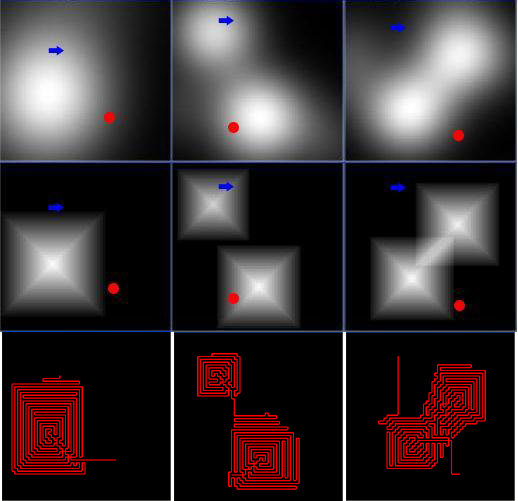
\includegraphics[width=6in]{maps900.jpg}
\caption{Top row: 2D representations of unimodal, bimodal, and bimodal with overlap probability distribution maps. Middle row: Simplified versions of the three types of maps. Bottom row: Best paths found for each map.}
\label{maps}
%\vspace*{-4ex}
\end{figure}


%=============================
\subsection{Experimental Results and Analysis}

For each distribution type (real and simplified maps) we ran each algorithm (with or without set destination) using $T$=120, 300, and 900 (4, 10, and 30 minutes). Because of random factors, we ran each experiment 10 times and calculated mean and standard deviation of the results. Due to space limitation, only a subset of the experimental results are presented (e.g. Table~\ref{EBimodalSimplified}, \ref{TBimodalSimplified} and Figure~\ref{graphBimodal}--\ref{graphRealSimple}).

For all the experiments we performed, algorithm running time exhibited the same trend: from the fastest to the slowest we have LHC-GW-CONV(\_E), EA(\_E) and LHC-GW-PF(\_E). For example, with the simplified unimodal map, the LHC-GW-PF algorithm ran for 9.419, 41.952 and 164.383 seconds for $T$=120, 300 and 900 respectively. Because the EA(\_E) algorithms use the path generated from other algorithms as seeds in the initial population, they are generally slower. However, most of the running time is spent generating the initial population and the evolutionary part of these algorithms only takes a fraction of a second. LHC-GW-PF(\_E) algorithms are always the slowest, and that is why we do not include them as seeds in the EA algorithms. For the group of algorithms with set destination, we perform path planning both from the starting node to the ending node and also from the ending node to the starting node (then reverse the path), and then select the better one; we include both runs when we record the algorithm running time. Therefore, the ``\_E'' algorithms always take more time to complete compared to the version before modification.

For the simplified unimodal map, the LHC-GW-CONV(\_E) algorithms are the clear winners in each respective group if we consider both the $\mathit{Efficiency}$ and the running time. For the group of algorithms without set destination, all algorithms gave above $99.5\%$ $\mathit{Efficiency}$. The LHC-GW-CONV algorithm is always the fastest  (e.g. 6.483 seconds for $T$=900) and achieved 100\% $\mathit{Efficiency}$ in all cases. The EA-Dir and EA-Path algorithms also achieved 100\% $\mathit{Efficiency}$, but at a much slower speed (e.g. 62.236 seconds for $T$=900 with EA-Path). For the group of algorithms with set destination, the LHC-GW-CONV\_E algorithm is also the fastest  (e.g. 14.173 seconds for $T$=900) and achieved 99.955\% or higher $\mathit{Efficiency}$ in all cases. Although the EA-Path\_E algorithm achieved slightly better $\mathit{Efficiency}$ (less than 0.1\% improvements), it did so at the cost of more running time (e.g. 78.334 seconds for $T$=900).

For the simplified bimodal map, the LHC-GW-CONV(\_E) algorithms did not always perform well because it doesn't handle the space between the two modes very well, especially for very short flight time. Fig.~\ref{graphBimodal} shows the $\mathit{Efficiency}$ comparison of the group of algorithms without set destination. The LHC-GW-PF(\_E) algorithms still achieved 96\% and above $\mathit{Efficiencies}$, but they are also the slowest. The EA(\_E) algorithms are more attractive in this case because they achieved the best $\mathit{Efficiencies}$ (98.095\%+ for EA and 97.857\%+ for EA\_E) very quickly.

\begin{table}
%\small
	\centering
		\begin{tabular}
			{|l|c|c|c|c|c|c|}
			\hline
			(\%) & \multicolumn{3}{|c|}{Simplified ({\it{Efficiency}})} & \multicolumn{3}{|c|}{Real ({\it{Efficiency$_\textrm{LB}$}})} \\
			\hline
			$T$ & 120 & 300 & 900	& 120 & 300 & 900 \\
			\hline
			LHC-GW-CONV & 88.89 & 96.80 & 98.35 & 81.64 & 93.97 & 97.75 \\
			\hline			
			LHC-GW-PF	& 96.63 & 96.70 & 96.07 & 90.28 & 92.43 & 96.67 \\ 
			\hline
			EA-Dir & 98.59 & 97.31 & 98.80 & 90.62 & 94.96 & 97.96 \\
			\hline
			EA-Path & 98.66 & 98.09 & 99.07 & 91.18 & 95.71 & 98.02 \\
			\hline
		\end{tabular}
\caption{Algorithm efficiency comparison for bimodal distribution}
\label{EBimodalSimplified}
%\vspace*{-5ex}
\end{table}

\begin{table}
	\centering
		\begin{tabular}
			{|l|c|c|c|c|c|c|}
			\hline
			(seconds) & \multicolumn{3}{|c|}{Simplified} & \multicolumn{3}{|c|}{Real} \\
			\hline
			$T$ & 120 & 300 & 900	& 120 & 300 & 900 \\
			\hline
			LHC-GW-CONV & 0.90 & 2.26 & 7.35 & 0.52 & 1.16 & 5.66 \\
			\hline
			LHC-GW-PF	& 9.44 & 29.11 & 131.35 & 2.61 & 8.64 & 92.38 \\
			\hline
			EA-Dir & 9.36 & 15.56 & 41.71 & 10.97 & 16.69 & 35.11 \\
			\hline
			EA-Path & 10.63 & 22.89 & 66.31 & 12.61 & 21.20 & 53.73 \\
			\hline
		\end{tabular}
\caption{Algorithm speed comparison for bimodal distribution}
\label{TBimodalSimplified}
%\vspace*{-7ex}
\end{table}

\begin{figure}
%\vspace*{-2ex}
\centering
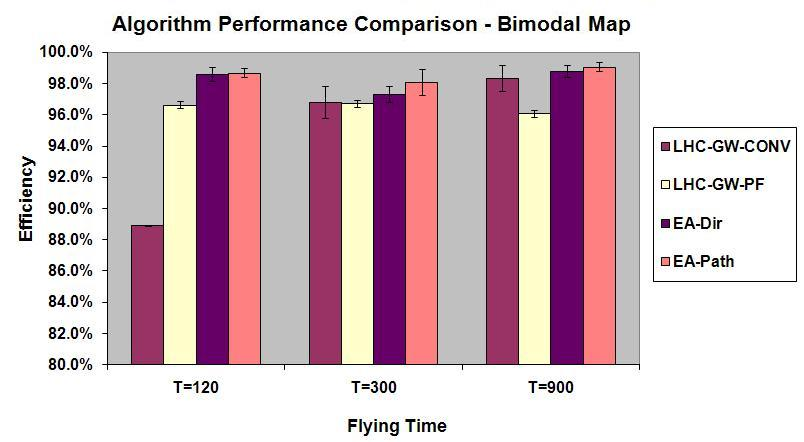
\includegraphics[width=6in]{graphBimodal.jpg}
\caption{$\mathit{Efficiency}$ comparison for group of algorithms without set destination for simplified bimodal map}
\label{graphBimodal}
%\vspace*{-2ex}
\end{figure}

For the simplified bimodal with overlap map, the EA(\_E) algorithms achieved the best $\mathit{Efficiencies}$ (98.302\%+ for EA and 98.653\%+ for EA\_E), but the LHC-GW-CONV(\_E) algorithms were able to achieve equivalent or slightly lower Efficiencies (97.391\%+ for LHC-GW-CONV and 98.429\%+ for LHC-GW-CONV\_E) with much less time (8.283 seconds and 16.296 seconds for $T$=900 respectively). Fig.~\ref{graphEBimodalOverlap} shows the $\mathit{Efficiency}$ comparison of the group of algorithms with set destination.

\begin{figure}
\centering
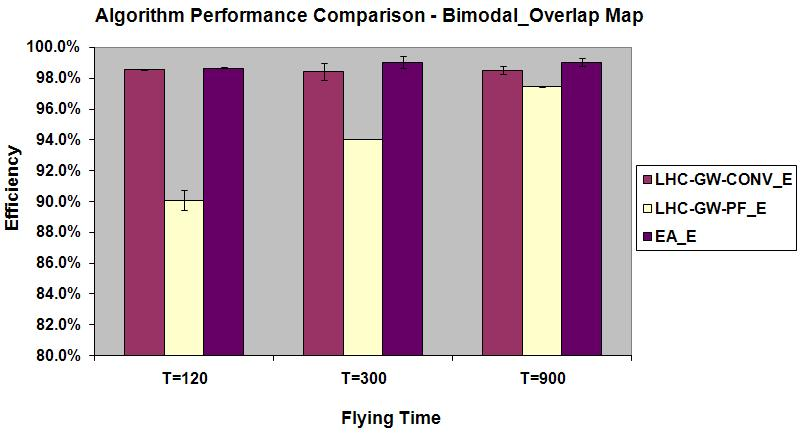
\includegraphics[width=6in]{graphEBimodalOverlap.jpg}
\caption{$\mathit{Efficiency}$ comparison for group of algorithms with set destination for simplified bimodal with overlap map}
\label{graphEBimodalOverlap}
%\vspace*{-4ex}
\end{figure}

For each of the three real distribution maps (unimodal, bimodal, and bimodal with overlap), since $PC_{p^*}$ is unknown, we can only calculate $\mathit{Efficiency_{LB}}$. We observed that the $\mathit{Efficiency_{LB}}$ for each real map is very close to the $\mathit{Efficiency_{LB}}$ for each of the counterpart simplified maps, and we hypothesize that the $\mathit{Efficiency}$ for each real map should also be close to the $\mathit{Efficiency}$ for each of the counterpart simplified maps. Fig.~\ref{graphRealSimple} shows an example of the EA-Path algorithm performance for the real and simplified bimodal with overlap map. The columns in the front row are $\mathit{Efficiency_{LB}}$ values and the columns in the back row are $\mathit{Efficiency}$ values. Based on this graph, we estimate that the $\mathit{Efficiency}$ values for the real map here are above 97\% for all $T$ values.

\begin{figure}
%\vspace*{-3ex}
\centering
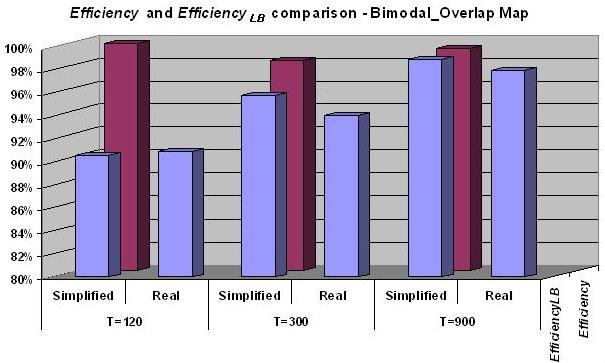
\includegraphics[width=6in]{graphRealSimple.jpg}
\caption{EA-Path performance for the real and simplified bimodal with overlap map}
\label{graphRealSimple}
\end{figure}

To further evaluate our algorithms, we tested our algorithms on a more complex multimodal distribution map generated by mixing multiple Gaussian distributions with various standard deviations; see Fig.~\ref{ComplexMap}. The LHC-GW-CONV algorithm achieved 97.206\% $\mathit{Efficiency_{LB}}$ in 5.516 seconds and the EA-Path algorithm achieved 97.609\% $\mathit{Efficiency_{LB}}$ in 63.984 seconds. Note here that the $\mathit{Efficiency}$ percentiles can only be better.

\begin{figure}
\centering
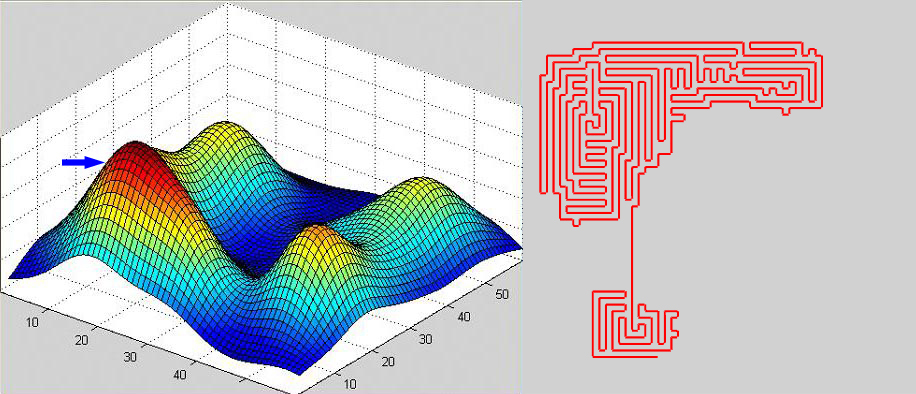
\includegraphics[width=6in]{ComplexMap3.jpg}
\caption{More complex multimodal probability distribution map}
\label{ComplexMap}
%\vspace*{-3ex}
\end{figure}

In every experiment, the EA(\_E) algorithms always achieved the best $\mathit{Efficiency}$ and $\mathit{Efficiency_{LB}}$. Therefore, if the operator has some time for computation, they seem to be attractive candidates. If the operator needs a path generated quickly, the LHC-GW-CONV(\_E) algorithms can be used. Although the LHC-GW-PF(\_E) algorithms do not work as well with these three distribution maps, initial tests on other distribution types such as sparse map and small-multimodal map suggest that they could perform better than other algorithms.


%=================================================================================	
\section{Conclusion and Future Work}

We model the UAV path planning problem in WiSAR as a discretized combinatorial optimization problem and design two groups of algorithms for path planning with or without a set destination using algorithms based on Local Hill Climbing, and Evolutionary Algorithms using novel techniques such as ``global warming effect'' and path crossover/mutation. We evaluate the performances of these algorithms on six (3 simplified, 3 ``real'') representations of typical WiSAR probability distribution maps, unimodal, bimodal, and bimodal with overlap, with various flight times and use the simplified maps to validate true efficiencies in real maps. Experimental results show that our algorithms can generate good paths with high $\mathit{Efficiency}$ or estimated $\mathit{Efficiency}$ that approximate the optimal solution within reasonable computation time. Specifically, the LHC-GW-CONV(\_E) algorithms should be used for unimodal maps, and if a few minutes computation time is available, because the EA(\_E) algorithms always keep the best path found from seed algorithms, they can always find a path with the highest $\mathit{Efficiency}$ compared with other algorithms experimented.

Experimenting with more types of distribution maps, designing a more advanced global warming search model, allowing 8-connected path planning, and dealing with dynamic distribution maps that change over time are all natural extensions for future work. Specifically, the set of algorithms with set destinations enables us to further investigate how the path planning task can be segmented so human operators can plan more strategically while the algorithms plan tactically, and what interface can make this an intuitive, smooth, and effective task for the UAV operator in WiSAR operations.
